% !TEX TS-program = Xelatex
% !TEX encoding = UTF-8 Unicode

\documentclass[UTF8]{ctexart}
\usepackage{amsmath}
\usepackage[bottom]{footmisc}
\usepackage{geometry}
\usepackage{graphicx}
\usepackage{figsize}
\usepackage[separate-uncertainty = true,per-mode=symbol]{siunitx}
\usepackage{tabu}
\usepackage{wasysym}
\geometry{left=0.7in,right=0.7in,bottom=0.7in,top=0.7in}

\title{实验十九:分光计的调节与掠入射法测量玻璃折射率}
\author{朱寅杰 1600017721}
\date{2017年11月17日}

\begin{document}

\maketitle

\subsection{测量三棱镜的顶角}
分别将望远镜对准三棱镜的两个光学面的法向,记录两个游标盘上角度的读数,有顶角$A=\pi-(\frac{\theta_2'+\theta_2}{2}-\frac{\theta_1'+\theta_1}{2})$。
\begin{center}
\noindent
\begin{tabu} to 0.7\linewidth {X[c,-1]|X[c,-10] X[c,-10]|X[c,-10] X[c,-10]||X[c]}
\hline
编号	&$\theta_1$	&$\theta_1'$	&$\theta_2$	&$\theta_2'$	&顶角$A$
\\
\hline
1	&\ang{181;14;}	&\ang{1;15;}	&\ang{301;14;}	&\ang{121;15;}	&\ang{60;0;0}
\\
2	&\ang{177;53;}	&\ang{357;53;}	&\ang{297;51;}	&\ang{117;52;}	&\ang{60;1;30}
\\
3	&\ang{311;55;}	&\ang{131;53;}	&\ang{71;56;}	&\ang{251;57;}	&\ang{59;57;30}
\\
\hline
\end{tabu}
\end{center}
取平均算出$\bar{A}=\ang{59;59;40}$,$\sigma_{\bar{A}}=\ang{;1;10}$。游标盘的允差取为\ang{;1;},对应一个\ang{;;35}的不确定度。二者合成,得$\sigma_A=\ang{;1;18}$,故$A=\num{1.0471(4)}$。

\subsection{掠入射法测量三棱镜玻璃的折射率}
使用钠黄光(波长为\SI{5893}{\nm})的扩展光源从接近切向的方位入射到棱镜,分别读取出射光学面的法向$\frac{\theta_2'+\theta_2}{2}$与视野中明暗分解位置$\frac{\theta_1'+\theta_1}{2}$,则出射的极限角等于$\phi=\pi-(\frac{\theta_2'+\theta_2}{2}-\frac{\theta_1'+\theta_1}{2})$。从这个极限角可以计算出折射率。
\begin{center}
\noindent
\begin{tabu} to 0.7\linewidth {X[c,-1]|X[c,-10] X[c,-10]|X[c,-10] X[c,-10]||X[c]}
\hline
编号	&$\theta_1$	&$\theta_1'$	&$\theta_2$	&$\theta_2'$	&极限出射角$\phi$
\\
\hline
1	&\ang{202;15;}	&\ang{22;16;}	&\ang{340;47;}	&\ang{160;47;}	&\ang{41;38;30}
\\
2	&\ang{154;7;}	&\ang{334;8;}	&\ang{292;43;}	&\ang{112;32;}	&\ang{41;30;0}
\\
3	&\ang{260;55;}	&\ang{80;55;}	&\ang{39;31;}	&\ang{219;32;}	&\ang{41;23;30}
\\
\hline
\end{tabu}
\end{center}
取平均算出$\bar{\phi}=\ang{41;30;40}$,$\sigma_{\bar{\phi}}=\ang{;4;21}$。游标盘的允差取为\ang{;1;},对应一个\ang{;;35}的不确定度。二者合成,得$\sigma_{\phi}=\ang{;4;23}$,故$\phi=\num{.7245(13)}$。
\[
n=\sqrt{1+(\frac{\cos{A}+\sin\phi}{\sin{A}})^2}=\num{1.674263936}
\]
\[
\sigma_n=\frac{\sqrt{n^2-1}}{n}\sqrt{(\frac{\sigma_A}{\sin^2A})^2+(\sigma_{\phi}\frac{\cos{\phi}}{\sin{A}})^2}=\num{9.5e-4}
\]
故有$n=\num{1.6742(9)}$。

\subsection{最小偏向角法测量三棱镜玻璃折射率}
将汞灯通过平行光管从切向入射棱镜,用望远镜找到折射色散出的分立谱线。缓缓转过棱镜的角度,同时望远镜紧跟视野中所测量的那条谱线,捕捉谱线在视野中由左而右再转向左中间转折的位置,读出其角度$\frac{\theta_1'+\theta_1}{2}$,再测出未经折射的白光的位置$\frac{\theta_2'+\theta_2}{2}$,则有最小偏向角$\delta=\pi-(\frac{\theta_2'+\theta_2}{2}-\frac{\theta_1'+\theta_1}{2})$。由各色光的最小偏向角即可计算出玻璃对各色光的折射率。
\begin{center}
\noindent
\begin{tabu} to 0.9\linewidth {X[c,-10]|X[c,-10] X[c,-10]|X[c,-10] X[c,-10]||X[c]|X[c]}
\hline
谱线波长	&$\theta_1$	&$\theta_1'$	&$\theta_2$	&$\theta_2'$	&最小偏向角$\delta$	&折射率计算值$n$
\\
\hline
\SI{407.78}{\nm}(紫)	&\ang{109;31;}	&\ang{289;31;}	&\ang{232;59;}	&\ang{52;58;}	&\ang{56;32;30}	&1.7012
\\
\SI{435.84}{\nm}(蓝)	&\ang{118;30;}	&\ang{298;31;}	&\ang{242;6;}	&\ang{62;5;}	&\ang{56;25;0}	&1.7000
\\
\SI{546.07}{\nm}(绿)	&\ang{117;37;}	&\ang{297;40;}	&\ang{243;25;}	&\ang{63;24;}	&\ang{54;14;0}	&1.6796
\\
	&\ang{224;21;}	&\ang{44;20;}	&\ang{350;5;}	&\ang{170;6;}	&\ang{54;15;0}	&1.6798
\\
	&\ang{277;30;}	&\ang{97;33;}	&\ang{43;18;}	&\ang{223;17;}	&\ang{54;14;0}	&1.6796
\\
\SI{579.07}{\nm}(黄)	&\ang{286;50;}	&\ang{106;48;}	&\ang{53;8;}	&\ang{233;8;}	&\ang{53;41;0}	&1.6744
\\
\SI{612.33}{\nm}(红)	&\ang{286;25;}	&\ang{106;25;}	&\ang{53;14;}	&\ang{233;15;}	&\ang{53;10;30}	&1.6695
\\
\hline
\end{tabu}
\end{center}
对\SI{546.07}{\nm}的绿线我们测了三次,以检验我们测量结果的可靠性。三次最小偏向角的平均值为$\bar{\delta}=\ang{54;14;20}$,此平均值的统计不确定度为$\sigma_{\bar{\delta}}=\ang{;;24}$,再计入游标盘\ang{;1;}的允差折算成的不确定度\ang{;;35},得$\delta$的不确定度$\sigma_{\delta}=\ang{;;42}$,有$\delta=\num{.9466(2)}$。得
\[
n=\sin{(A+\delta)/2}/\sin{(A/2)}=\num{1.67970}
\]
\[
\sigma_n=\frac{1}{2\sin{(A/2)}}\sqrt{(\sigma_A\frac{\sin{(\delta/2)}}{\sin{(A/2)}})^2+(\sigma_{\delta}\cos{\frac{A+\delta}{2}})^2}=\num{3.6e-4}
\]
故对绿线$n=\num{1.6797(4)}$。我们测量的精度还是比较好的。

将不同波长下折射率的数值按书上给出的正常色散的柯西公式拟合,得到
\[n=(\num{1.602(8)})+\SI{3.2(4)e4}{\nm\squared}/\lambda^2-\SI{2.5(5)e9}{nm^4}/\lambda^4\]
拟合的曲线见下图。几个系数的统计不确定度(由软件自动算出标准偏差)还是相当大的,固然有所测波长范围较窄、数据点较少的原因,但是主要还是测量不够精细导致。做的时候时间比较紧,所以各条线测得都比较仓促,其他几条线也没有像绿线一样重复测三次,可能会有游标读数不准,或者螺丝锁得不完全紧之类的情况。还请老师包涵。
\begin{center}
	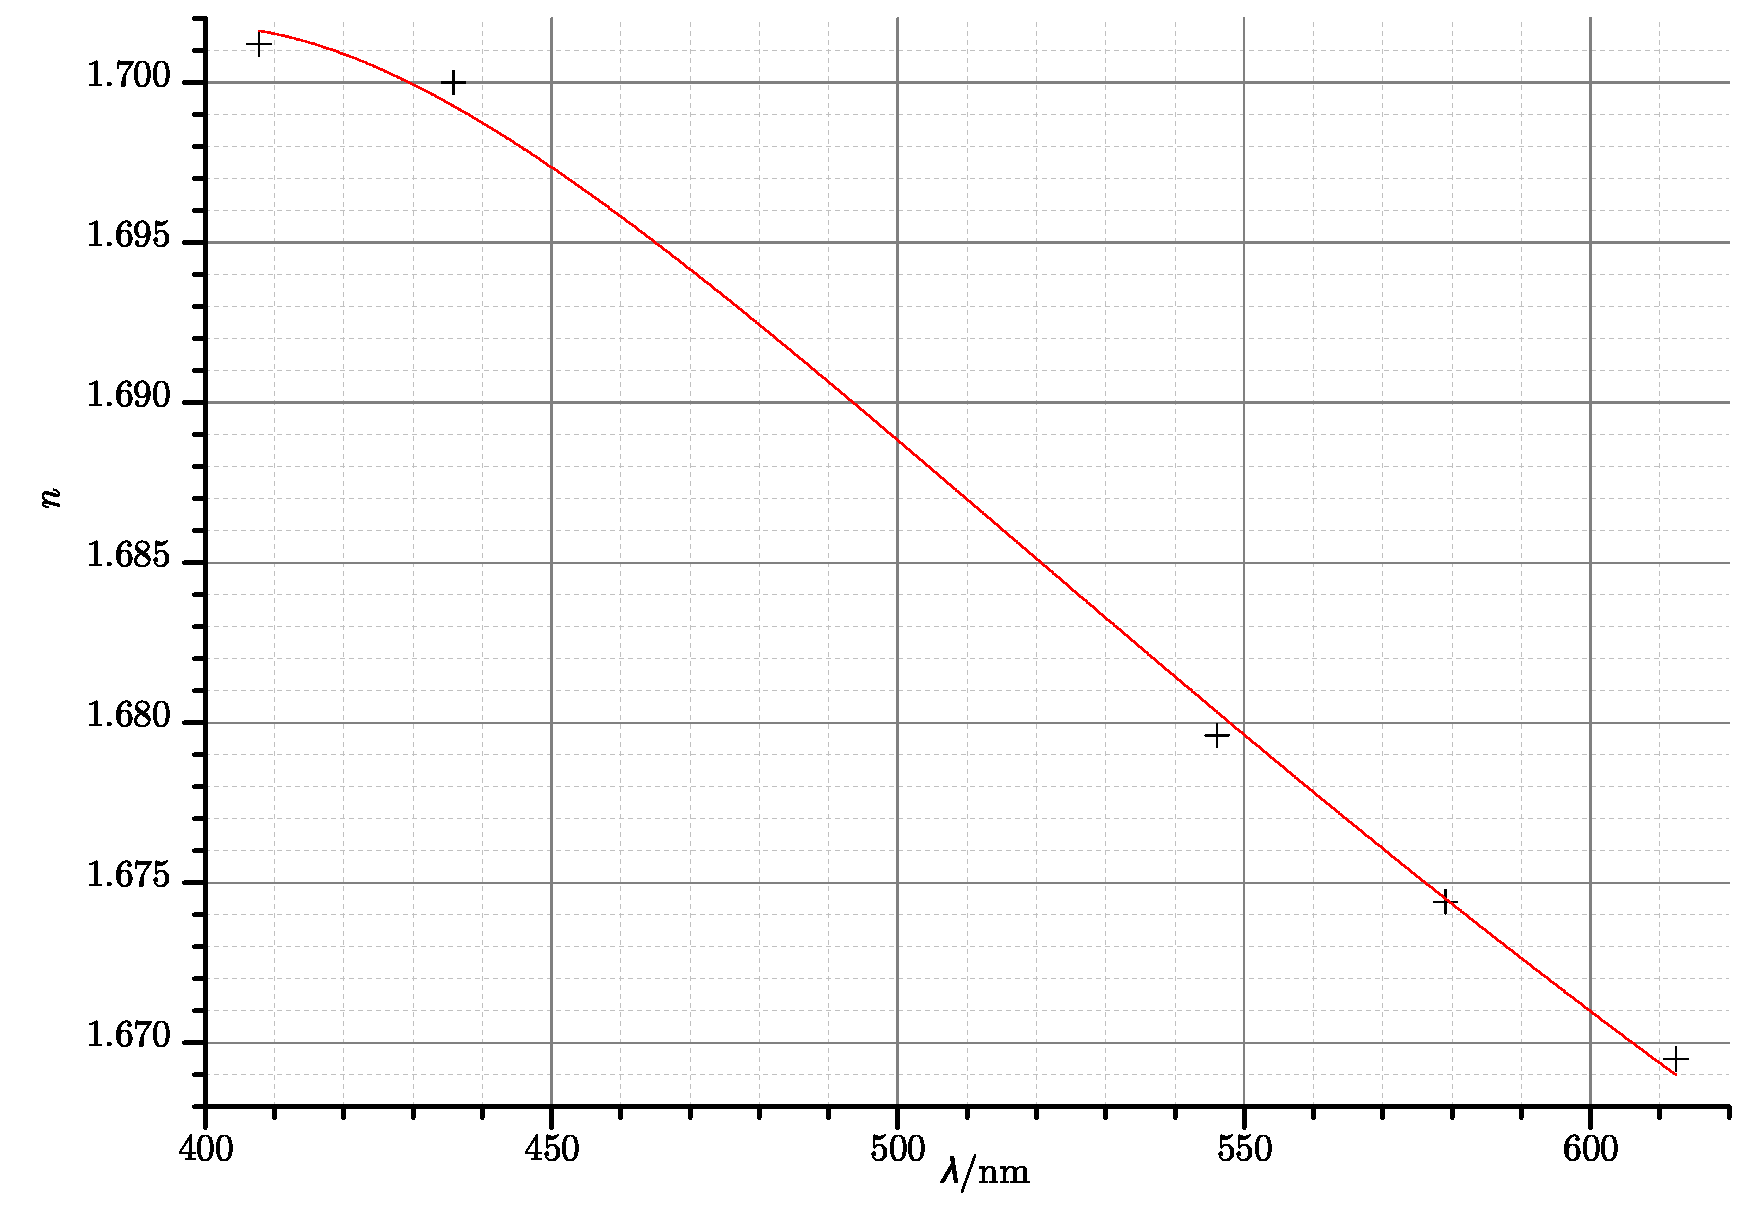
\includegraphics[width=0.9\linewidth,keepaspectratio=true]{Dispersion.eps}
\end{center}
\end{document} 